\documentclass{article}

\usepackage{graphicx}
\usepackage{cite}
\usepackage[margin=1in]{geometry}
\usepackage{hyperref}

\begin{document}


\title{MicroDB Graph Database}

\author{Sreenivas Appasani \\ Ajay Mandlekar \\ Ruthwick Pathireddy \\ Sathwick Pathireddy \\
\\ CS123 Database Systems Project
\\ \it{California Institute of Technology}}

\maketitle

\section{Motivation}

Information is connected in the world and relationships are a central aspect of modeling such data. Traditional Relational Database Management Systems (RDBMS) model relationships through join-like operations, which are computationally intensive. There needs to be an efficient way to express relationships between large sets of data. Graph databases fulfill such a need and are a powerful alternative to relational databases. 

\section{Query Language}

MicroDB's Query Language supports both basic and commonly-used graph queries as listed below:
\begin{itemize}
	\item Create, modify, and delete nodes.
	\item Create, modify, and delete edges.
	\item Query for arbitrary length node-edge path relationships.
	\item Determine if a path exists between two nodes. 
	\item Find the shortest path between two nodes. 
\end{itemize}

% Mention that nodes are internally dictionaries with ids, edges are etc..

\subsection{Internal Data Structures}

Our graph database utilizes the networkx package \cite{nx} to maintain a graph representation in memory during an active database session. The graph infrastructure provided by this package is used to create and manipulate nodes and edges during an interactive user session. 

\subsection{Nodes}

Internally, each node is assigned a unique identifier, which is just a number. Each node's attributes is stored in a dictionary with attribute names as keys and attributes as values. When a query returns a set of nodes, the nodes are returned as a list of tuple pairs which contain its unique identifier and its dictionary of attributes. 

\subsubsection{Example Queries}

\noindent The following query creates a node which has attributes "Label", "Name", and "Salary".  

\begin{center} \textbf{CREATE n: id1 Label:Boss Name:Donnie Salary:1000000;} \end{center}

\begin{center} \textit{In this query, "id1" is simply a local identifier that can be used to refer to the created node by the user. The user can view the results that are stored in any given identifier by using the RETURN command (for example, RETURN id1;). Another useful command for viewing the current contents of the in-memory graph is the SHOW command. It might be a good idea to run a SHOW command after every one of the following commands.} \end{center}

\noindent The following query modifies the existing node's attributes. 

\begin{center} \textbf{MODIFYNODE n: prev Name:Donnie n: new Name:Ruthwick b: new val:1;} \end{center}

\begin{center} \textit{In this case, only the "Name" attribute is modified. It should be noted that this command will match on all nodes whose "Name" attribute is "Donnie" and update their "Name" attribute to be "Ruthwick". This allows for a simple mechanism to update several related nodes at once. The important part of the "b:" portion of the query is the value of 1. This value is a boolean flag that indicates whether the attribute is to be updated or deleted. If this flag had been set to 0, the "Name" attribute would have been deleted (the new "Name" value would have been irrelevant). The other fields present in the "b:" part of the query are dummy fields that are necessary for the parser. Note that both "prev" and "new" are both identifiers just as "id1" in the create node query above.} \end{center}

\noindent The following query deletes the node.

\begin{center} \textbf{DELETENODE n: fst Name:Donnie;} \end{center}

\begin{center} \textit{In particular, the query deletes all nodes whose "Name" attribute is "Donnie". Once again, "fst" is used as an identifier. However, the identifier serves no purpose here. It is included for ease of parsing.} \end{center}

\subsection{Edges}

\noindent Internally, each edge is stored in a dictionary that uses the two node identifiers as a key and the relationship attributes as a value. When an edge is queried, the result is represented as a tuple triple which consists of two node identifiers and a dictionary of attributes that describe the relationship. The keys in the dictionary are edge attribute names and the values are the edge attributes. 

\subsubsection{Example Queries}

\noindent Let's continue the previous example. We first create a second node.

\begin{center} \textbf{CREATE n: id2 Label:Employee Name:Sreeni Salary:50000;} \end{center}

\noindent Then, we create an edge between the nodes. 

\begin{center} \textbf{CREATEEDGE n: id1 Label:Boss e: id3 Relation:Manager n: id2 Label:Employee;} \end{center}

\begin{center} \textit{The command creates an edge between all nodes whose "Label" attribute is "Boss" and all nodes whose "Label" attribute is "Employee". The edge has an attribute called "Relation" and the value is set to "Manager". Note that this is a directed edge from the first node to the second node.} \end{center}

\noindent The following query modifies the edge by changing its attribute.

\begin{center} \textbf{MODIFYEDGE e: fst Relation:Manager e: snd Relation:Co-worker b: oth val:1;} \end{center}

\begin{center} \textit{This command works just like the MODIFYNODE command. It updates all edges with "Relation" fields equal to "Manager" to set their fields to "Co-worker".} \end{center}

\noindent The following query deletes the edge we just created. 

\begin{center} \textbf{DELETEEDGE e: a Relation:Co-worker;} \end{center}

\begin{center} \textit{This command deletes all edges whose "Relation" field is equal to "Co-worker".} \end{center}

\subsection{Match Query}

\noindent Match queries are used to query for arbitrary length node-edge-node relationships. It can also be used to query for a single type of node or a single type of edge. The internal process used to match a single node or single edge simply involves a networks dictionary lookup. For arbitrary length relationships, we implemented an algorithm that repeatedly utilizes set intersection on node-edge-node triples in the path until we collapse the nodes to our desired result.

\subsubsection{Example Queries}

\noindent The following query matches a single node with the following attributes.

\begin{center} \textbf{MATCH n: id1 Animal:Dog;} \end{center}

\begin{center} \textit{The command finds nodes with the attribute key "Animal" whose value is "Dog".} \end{center}

\noindent The following query matches a single edge with the following attributes.

\begin{center} \textbf{MATCH e: id2 Relation:Enemy;} \end{center}

\begin{center} \textit{The command finds edges that contain an attribute key "Relation" whose value is "Enemy".} \end{center}

\noindent The following query matches a node-edge-node path with some attributes.

\begin{center} \textbf{MATCH n: id1 Animal:Dog e: id2 Relation:Enemy n: id3 Age:10;} \end{center}

\begin{center} \textit{The command finds nodes that not only have the attribute dictionary {"Animal" : "Dog"} but is also connected to an edge with "Relation" type Enemy which is connected to another node with an attribute dictionary {"Age":10}. } \end{center}

\subsection{Graph Functionality}

In addition to basic creation, deletion, and matching of nodes and edges, MicroDB provides functionality to perform common graph operations. Most of these operations are implemented as an abstraction on top of the graph library operations the networkx package provides. Other operations are provided to ease user experience during an interactive session.   

\subsubsection{Example Operations}

\noindent The following operation determines is a path exists between two nodes specified by the given attributes. 

\begin{center} \textbf{HASPATH n: id1 Name:Ruff n: id2 Name:Furry;} \end{center} 

\begin{center} \textit{In this query, we want to find out if there is a path between a node with name "Ruff" and a node with name "Furry".} \end{center}

\noindent The following operation displays the shortest path between the two nodes if it exists. If no path exists, a message is displayed to the user.

\begin{center} \textbf{SHORTESTPATH n: id1 Name:Ruff n: id2 Name:Furry;} \end{center} 

\begin{center} \textit{In this query, we display the shortest path between a node with name "Ruff" and a node with name "Furry".} \end{center}

\noindent The following operation returns a all neighbors of nodes that contain some specific attributes.

\begin{center} \textbf{NEIGHBOR n: id1 Name:Ruff;} \end{center} 

\begin{center} \textit{In this query, we want to know all the neighbors of the node with name "Ruff".} \end{center}

\noindent The following operation determines if an edge exists between two nodes specified by the given attributes.

\begin{center} \textbf{HASEDGE n: id1 Name:Ruff n: id2 Name:Furry;} \end{center} 

\begin{center} \textit{In this query, we want to know if there is a directed edge from the node with name "Ruff" to the node with name "Furry".} \end{center}

\noindent The following operation returns the value stored in an identifier.

\begin{center} \textbf{RETURN n: id1;} \end{center} 

\begin{center} \textit{The operation displays the value stored in the identifier id1.} \end{center}

\noindent The following operation displays the nodes, edges, and identifiers in the current session of the user.

\begin{center} \textbf{SHOW;} \end{center} 

\noindent The following operation clear all the contents of MicroDB.

\begin{center} \textbf{CLEAR;} \end{center} 

\noindent The following operation plots the contents of MicroDB using the matplotlib\cite{matplot} library.

\begin{center} \textbf{VISUALIZE;} \end{center} 



\section{Database System Architecture}

\subsection{Overview}

The following diagram describes interactions between major components of the system architecture as well as the files that pertain to each component. \\ \\ 

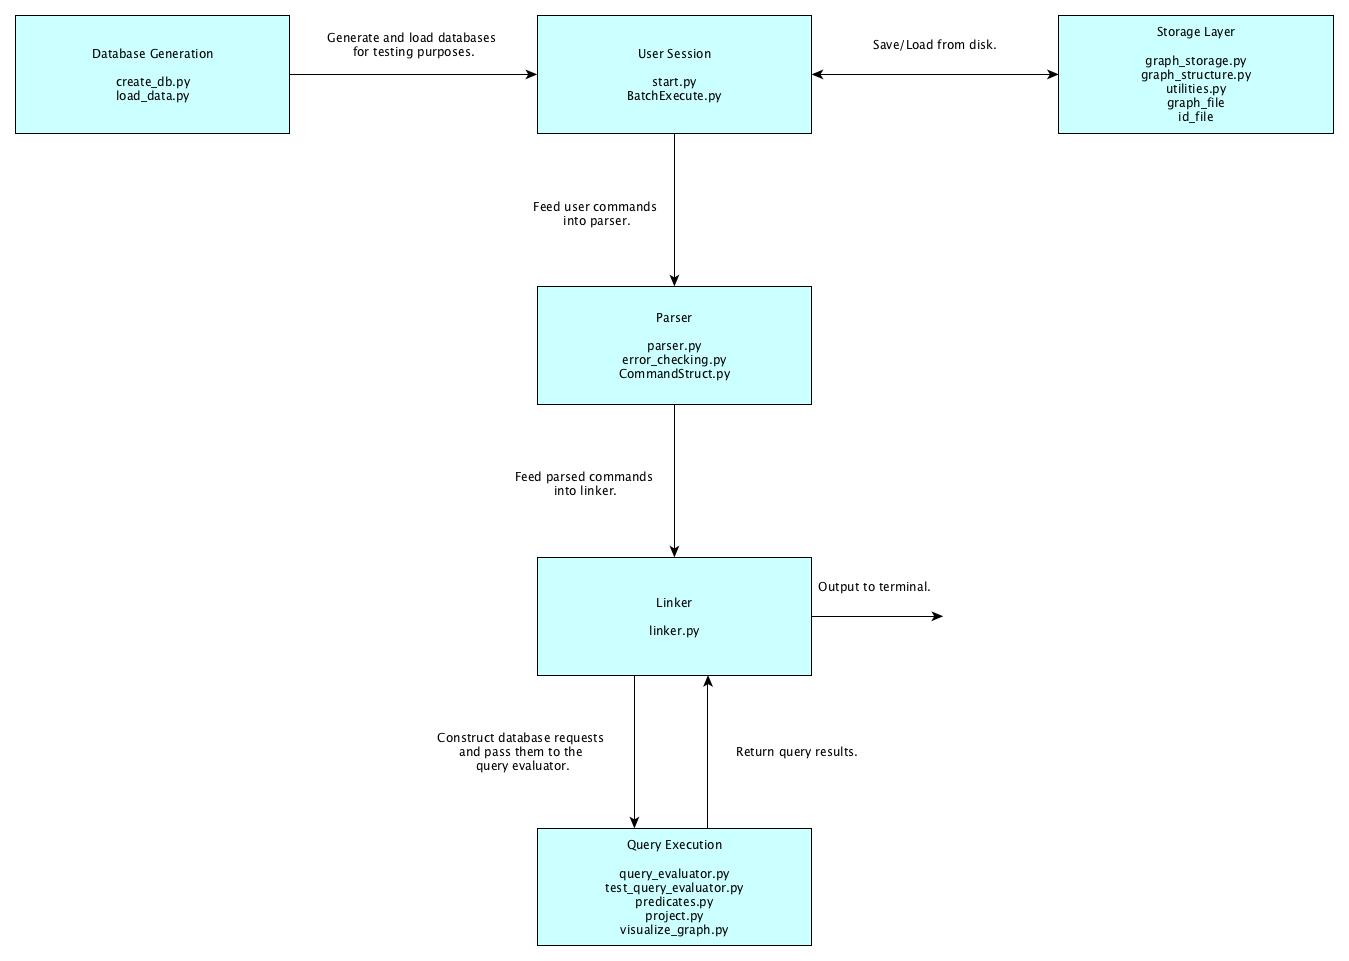
\includegraphics[width=16cm]{fileflow.jpg}

% TODO: Description of Overview

\subsection{User Interface}

\subsubsection{Files}

\begin{itemize}
	\item start.py - the main program that starts the database and handles all user interaction. 
	\item BatchExecute.py - allows the user to run a batch of commands from a text file.
\end{itemize}

% TODO: Description of UI

\subsection{Parser}

\subsubsection{Files}

\begin{itemize}
	\item parser.py - contains the main parser implementation.
	\item error\_checking.py - error checking functionality used by the parser. 
	\item CommandStruct.py - wrapper around commands for the parser, it also details all of the commands and their syntax. 
\end{itemize}

% TODO: Description of Parser 

\subsection{Linker}

\subsubsection{Files}

\begin{itemize}
	\item linker.py - contains the entire linker implementation. 
\end{itemize}

% TODO: Description of Linker 

\subsection{Query Evaluator}

\subsubsection{Files}

\begin{itemize}
	\item query\_evaluator.py - responsible for servicing all queries.
	\item test\_query\_evaluator.py - unit testing framework for servicing queries.
	\item predicates.py - responsible for processing predicates. 
	\item project.py - responsible for executing project operations. 
	\item visualize\_graph.py - produces a neat visualization of the database. Essentially responsible for executing the visualize command. 
\end{itemize}

% TODO: Description of Query Evaluator 

\subsection{Graph Storage}

\subsubsection{Files}

\begin{itemize}
	\item graph\_storage.py - contains the basic storage layer for loading the database from disk and writing the database to disk. 
	\item graph\_structure.py - contains the in-memory graph structure implementation, with the help of the networkx package. 
	\item utilities.py - miscellaneous useful functions for file I/O. 
	\item graph\_file - file that contains the entire database on disk.
	\item id\_file - file that saves the last unique identifier generated by the database on disk. 
\end{itemize}

% TODO: Description of Graph Storage 

\subsection{Testing}

\noindent To run tests, run the following command: \textbf{python test\_query\_evaluator.py} 

\begin{thebibliography}{10}

\bibitem{nx} Aric A. Hagberg, Daniel A. Schult and Pieter J. Swart, "Exploring network structure, dynamics, and function using NetworkX", in Proceedings of the 7th Python in Science Conference (SciPy2008), G�el Varoquaux, Travis Vaught, and Jarrod Millman (Eds), (Pasadena, CA USA), pp. 11-15, Aug 2008

\bibitem{matplot} J. D. Hunter. Matplotlib: A 2d graphics environment. Computing In Science \& Engineering, 9(3):90?95, 2007.

\end{thebibliography}


Link to Github Repository: \url{https://github.com/Sreeni34/DropDatabase}


\end{document}